\documentclass[1p]{elsarticle_modified}
%\bibliographystyle{elsarticle-num}

%\usepackage[colorlinks]{hyperref}
%\usepackage{abbrmath_seonhwa} %\Abb, \Ascr, \Acal ,\Abf, \Afrak
\usepackage{amsfonts}
\usepackage{amssymb}
\usepackage{amsmath}
\usepackage{amsthm}
\usepackage{scalefnt}
\usepackage{amsbsy}
\usepackage{kotex}
\usepackage{caption}
\usepackage{subfig}
\usepackage{color}
\usepackage{graphicx}
\usepackage{xcolor} %% white, black, red, green, blue, cyan, magenta, yellow
\usepackage{float}
\usepackage{setspace}
\usepackage{hyperref}

\usepackage{tikz}
\usetikzlibrary{arrows}

\usepackage{multirow}
\usepackage{array} % fixed length table
\usepackage{hhline}

%%%%%%%%%%%%%%%%%%%%%
\makeatletter
\renewcommand*\env@matrix[1][\arraystretch]{%
	\edef\arraystretch{#1}%
	\hskip -\arraycolsep
	\let\@ifnextchar\new@ifnextchar
	\array{*\c@MaxMatrixCols c}}
\makeatother %https://tex.stackexchange.com/questions/14071/how-can-i-increase-the-line-spacing-in-a-matrix
%%%%%%%%%%%%%%%

\usepackage[normalem]{ulem}

\newcommand{\msout}[1]{\ifmmode\text{\sout{\ensuremath{#1}}}\else\sout{#1}\fi}
%SOURCE: \msout is \stkout macro in https://tex.stackexchange.com/questions/20609/strikeout-in-math-mode

\newcommand{\cancel}[1]{
	\ifmmode
	{\color{red}\msout{#1}}
	\else
	{\color{red}\sout{#1}}
	\fi
}

\newcommand{\add}[1]{
	{\color{blue}\uwave{#1}}
}

\newcommand{\replace}[2]{
	\ifmmode
	{\color{red}\msout{#1}}{\color{blue}\uwave{#2}}
	\else
	{\color{red}\sout{#1}}{\color{blue}\uwave{#2}}
	\fi
}

\newcommand{\Sol}{\mathcal{S}} %segment
\newcommand{\D}{D} %diagram
\newcommand{\A}{\mathcal{A}} %arc


%%%%%%%%%%%%%%%%%%%%%%%%%%%%%5 test

\def\sl{\operatorname{\textup{SL}}(2,\Cbb)}
\def\psl{\operatorname{\textup{PSL}}(2,\Cbb)}
\def\quan{\mkern 1mu \triangleright \mkern 1mu}

\theoremstyle{definition}
\newtheorem{thm}{Theorem}[section]
\newtheorem{prop}[thm]{Proposition}
\newtheorem{lem}[thm]{Lemma}
\newtheorem{ques}[thm]{Question}
\newtheorem{cor}[thm]{Corollary}
\newtheorem{defn}[thm]{Definition}
\newtheorem{exam}[thm]{Example}
\newtheorem{rmk}[thm]{Remark}
\newtheorem{alg}[thm]{Algorithm}

\newcommand{\I}{\sqrt{-1}}
\begin{document}

%\begin{frontmatter}
%
%\title{Boundary parabolic representations of knots up to 8 crossings}
%
%%% Group authors per affiliation:
%\author{Yunhi Cho} 
%\address{Department of Mathematics, University of Seoul, Seoul, Korea}
%\ead{yhcho@uos.ac.kr}
%
%
%\author{Seonhwa Kim} %\fnref{s_kim}}
%\address{Center for Geometry and Physics, Institute for Basic Science, Pohang, 37673, Korea}
%\ead{ryeona17@ibs.re.kr}
%
%\author{Hyuk Kim}
%\address{Department of Mathematical Sciences, Seoul National University, Seoul 08826, Korea}
%\ead{hyukkim@snu.ac.kr}
%
%\author{Seokbeom Yoon}
%\address{Department of Mathematical Sciences, Seoul National University, Seoul, 08826,  Korea}
%\ead{sbyoon15@snu.ac.kr}
%
%\begin{abstract}
%We find all boundary parabolic representation of knots up to 8 crossings.
%
%\end{abstract}
%\begin{keyword}
%    \MSC[2010] 57M25 
%\end{keyword}
%
%\end{frontmatter}

%\linenumbers
%\tableofcontents
%
\newcommand\colored[1]{\textcolor{white}{\rule[-0.35ex]{0.8em}{1.4ex}}\kern-0.8em\color{red} #1}%
%\newcommand\colored[1]{\textcolor{white}{ #1}\kern-2.17ex	\textcolor{white}{ #1}\kern-1.81ex	\textcolor{white}{ #1}\kern-2.15ex\color{red}#1	}

{\Large $\underline{12n_{0169}~(K12n_{0169})}$}

\setlength{\tabcolsep}{10pt}
\renewcommand{\arraystretch}{1.6}
\vspace{1cm}\begin{tabular}{m{100pt}>{\centering\arraybackslash}m{274pt}}
\multirow{5}{120pt}{
	\centering
	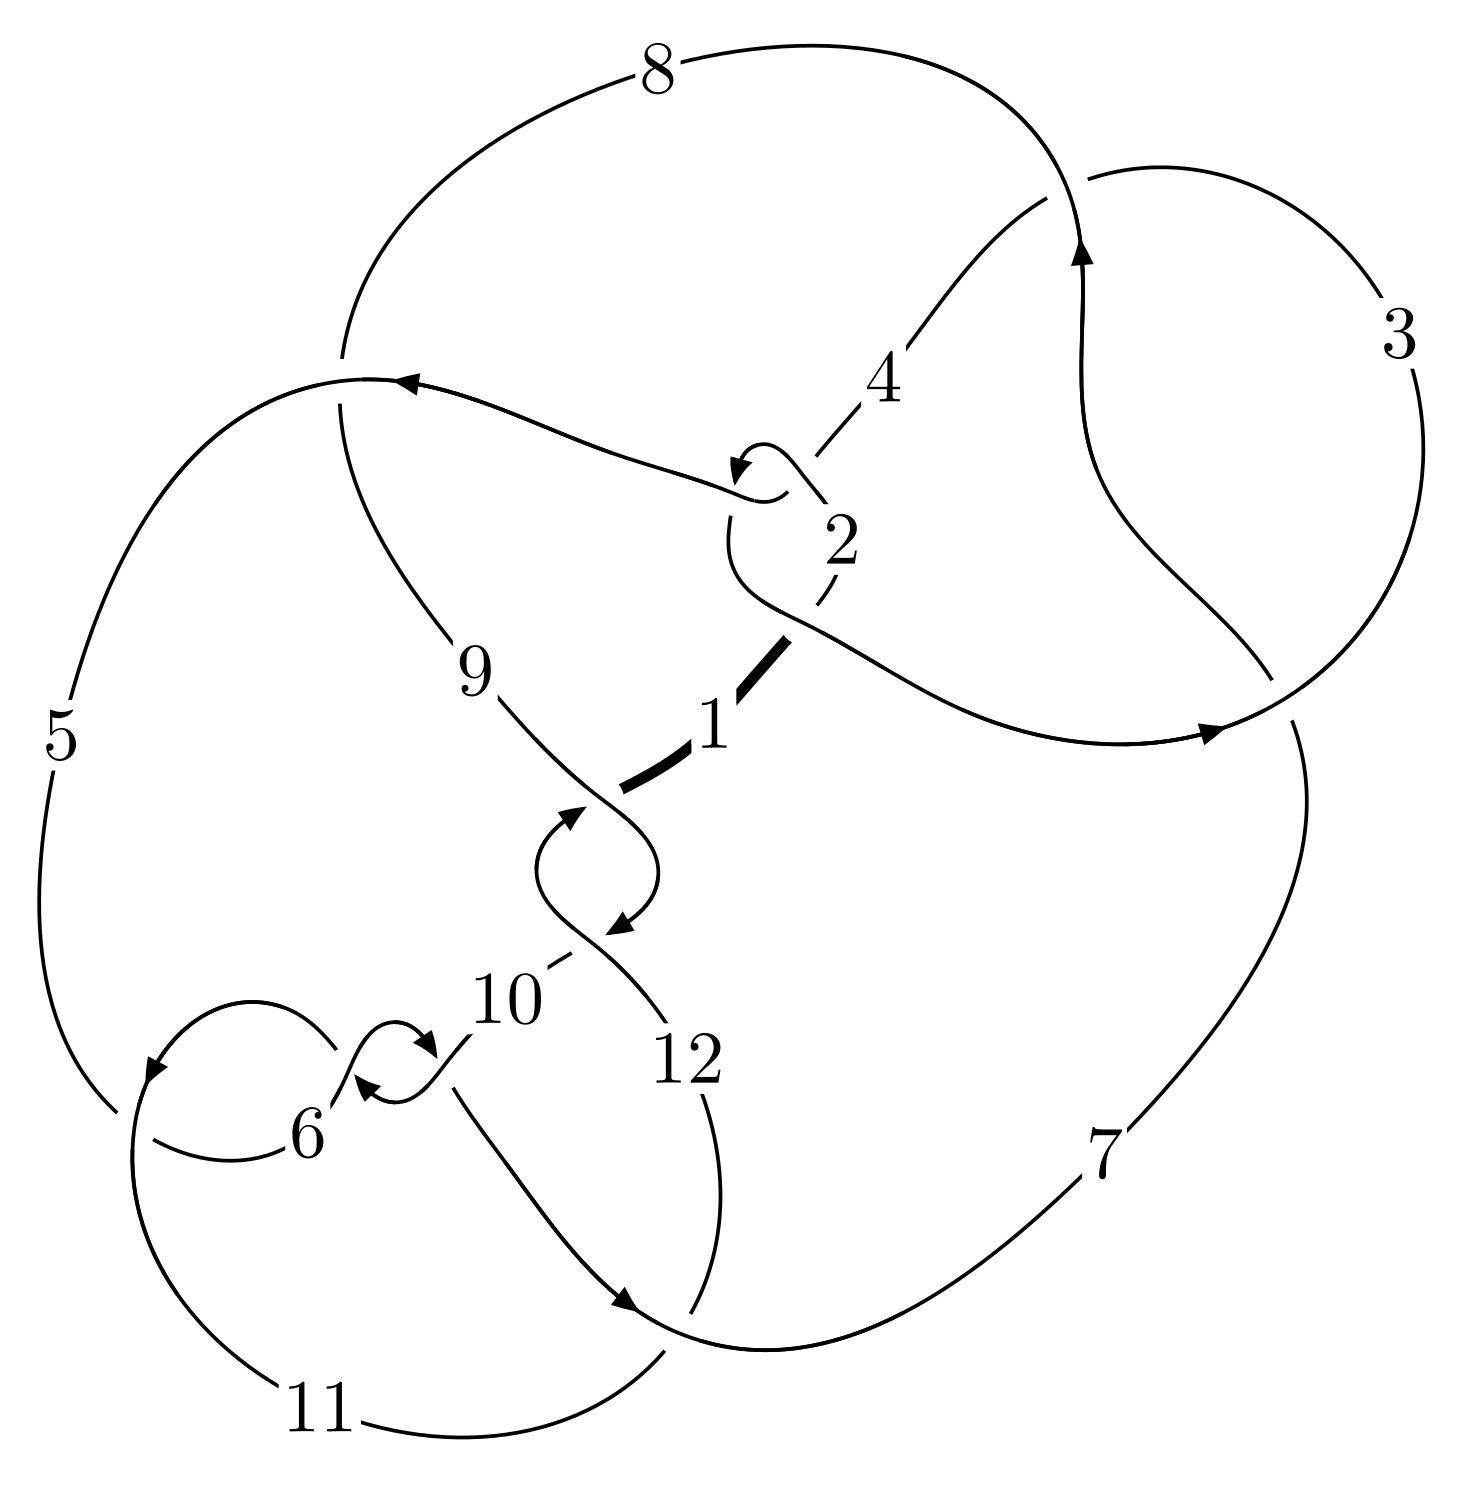
\includegraphics[width=112pt]{../../../GIT/diagram.site/Diagrams/png/2258_12n_0169.png}\\
\ \ \ A knot diagram\footnotemark}&
\allowdisplaybreaks
\textbf{Linearized knot diagam} \\
\cline{2-2}
 &
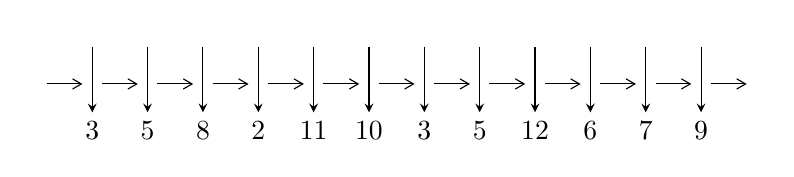
\begin{tikzpicture}[x=20pt, y=17pt]
	% nodes
	\node (C0) at (0, 0) {};
	\node (C1) at (1, 0) {};
	\node (C1U) at (1, +1) {};
	\node (C1D) at (1, -1) {3};

	\node (C2) at (2, 0) {};
	\node (C2U) at (2, +1) {};
	\node (C2D) at (2, -1) {5};

	\node (C3) at (3, 0) {};
	\node (C3U) at (3, +1) {};
	\node (C3D) at (3, -1) {8};

	\node (C4) at (4, 0) {};
	\node (C4U) at (4, +1) {};
	\node (C4D) at (4, -1) {2};

	\node (C5) at (5, 0) {};
	\node (C5U) at (5, +1) {};
	\node (C5D) at (5, -1) {11};

	\node (C6) at (6, 0) {};
	\node (C6U) at (6, +1) {};
	\node (C6D) at (6, -1) {10};

	\node (C7) at (7, 0) {};
	\node (C7U) at (7, +1) {};
	\node (C7D) at (7, -1) {3};

	\node (C8) at (8, 0) {};
	\node (C8U) at (8, +1) {};
	\node (C8D) at (8, -1) {5};

	\node (C9) at (9, 0) {};
	\node (C9U) at (9, +1) {};
	\node (C9D) at (9, -1) {12};

	\node (C10) at (10, 0) {};
	\node (C10U) at (10, +1) {};
	\node (C10D) at (10, -1) {6};

	\node (C11) at (11, 0) {};
	\node (C11U) at (11, +1) {};
	\node (C11D) at (11, -1) {7};

	\node (C12) at (12, 0) {};
	\node (C12U) at (12, +1) {};
	\node (C12D) at (12, -1) {9};
	\node (C13) at (13, 0) {};

	% arrows
	\draw[->,>={angle 60}]
	(C0) edge (C1) (C1) edge (C2) (C2) edge (C3) (C3) edge (C4) (C4) edge (C5) (C5) edge (C6) (C6) edge (C7) (C7) edge (C8) (C8) edge (C9) (C9) edge (C10) (C10) edge (C11) (C11) edge (C12) (C12) edge (C13) ;	\draw[->,>=stealth]
	(C1U) edge (C1D) (C2U) edge (C2D) (C3U) edge (C3D) (C4U) edge (C4D) (C5U) edge (C5D) (C6U) edge (C6D) (C7U) edge (C7D) (C8U) edge (C8D) (C9U) edge (C9D) (C10U) edge (C10D) (C11U) edge (C11D) (C12U) edge (C12D) ;
	\end{tikzpicture} \\
\hhline{~~} \\& 
\textbf{Solving Sequence} \\ \cline{2-2} 
 &
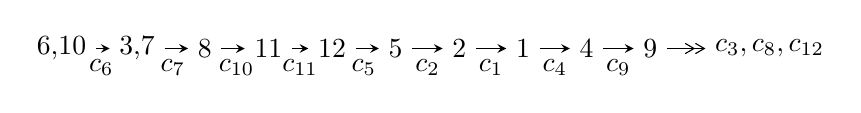
\begin{tikzpicture}[x=23pt, y=7pt]
	% node
	\node (A0) at (-1/8, 0) {6,10};
	\node (A1) at (17/16, 0) {3,7};
	\node (A2) at (17/8, 0) {8};
	\node (A3) at (25/8, 0) {11};
	\node (A4) at (33/8, 0) {12};
	\node (A5) at (41/8, 0) {5};
	\node (A6) at (49/8, 0) {2};
	\node (A7) at (57/8, 0) {1};
	\node (A8) at (65/8, 0) {4};
	\node (A9) at (73/8, 0) {9};
	\node (C1) at (1/2, -1) {$c_{6}$};
	\node (C2) at (13/8, -1) {$c_{7}$};
	\node (C3) at (21/8, -1) {$c_{10}$};
	\node (C4) at (29/8, -1) {$c_{11}$};
	\node (C5) at (37/8, -1) {$c_{5}$};
	\node (C6) at (45/8, -1) {$c_{2}$};
	\node (C7) at (53/8, -1) {$c_{1}$};
	\node (C8) at (61/8, -1) {$c_{4}$};
	\node (C9) at (69/8, -1) {$c_{9}$};
	\node (A10) at (11, 0) {$c_{3},c_{8},c_{12}$};

	% edge
	\draw[->,>=stealth]	
	(A0) edge (A1) (A1) edge (A2) (A2) edge (A3) (A3) edge (A4) (A4) edge (A5) (A5) edge (A6) (A6) edge (A7) (A7) edge (A8) (A8) edge (A9) ;
	\draw[->>,>={angle 60}]	
	(A9) edge (A10);
\end{tikzpicture} \\ 

\end{tabular} \\

\footnotetext{
The image of knot diagram is generated by the software ``\textbf{Draw programme}" developed by Andrew Bartholomew(\url{http://www.layer8.co.uk/maths/draw/index.htm\#Running-draw}), where we modified some parts for our purpose(\url{https://github.com/CATsTAILs/LinksPainter}).
}\phantom \\ \newline 
\centering \textbf{Ideals for irreducible components\footnotemark of $X_{\text{par}}$} 
 
\begin{align*}
I^u_{1}&=\langle 
- u^{31}+u^{30}+\cdots+b+2 u,\;u^{31}- u^{30}+\cdots+a-5 u,\;u^{32}-2 u^{31}+\cdots+5 u-1\rangle \\
I^u_{2}&=\langle 
b+u,\;u^2+a+2,\;u^3+2 u-1\rangle \\
I^u_{3}&=\langle 
- u^2+b- u,\;u^3+u^2+a+2 u+1,\;u^4+u^3+2 u^2+2 u+1\rangle \\
\\
\end{align*}
\raggedright * 3 irreducible components of $\dim_{\mathbb{C}}=0$, with total 39 representations.\\
\footnotetext{All coefficients of polynomials are rational numbers. But the coefficients are sometimes approximated in decimal forms when there is not enough margin.}
\newpage
\renewcommand{\arraystretch}{1}
\centering \section*{I. $I^u_{1}= \langle - u^{31}+u^{30}+\cdots+b+2 u,\;u^{31}- u^{30}+\cdots+a-5 u,\;u^{32}-2 u^{31}+\cdots+5 u-1 \rangle$}
\flushleft \textbf{(i) Arc colorings}\\
\begin{tabular}{m{7pt} m{180pt} m{7pt} m{180pt} }
\flushright $a_{6}=$&$\begin{pmatrix}1\\0\end{pmatrix}$ \\
\flushright $a_{10}=$&$\begin{pmatrix}0\\u\end{pmatrix}$ \\
\flushright $a_{3}=$&$\begin{pmatrix}- u^{31}+u^{30}+\cdots-7 u^2+5 u\\u^{31}- u^{30}+\cdots+3 u^2-2 u\end{pmatrix}$ \\
\flushright $a_{7}=$&$\begin{pmatrix}1\\u^2\end{pmatrix}$ \\
\flushright $a_{8}=$&$\begin{pmatrix}u^{13}+6 u^{11}+13 u^9+12 u^7+6 u^5+4 u^3+u\\- u^{13}-5 u^{11}-7 u^9+2 u^5-3 u^3+u\end{pmatrix}$ \\
\flushright $a_{11}=$&$\begin{pmatrix}- u\\u\end{pmatrix}$ \\
\flushright $a_{12}=$&$\begin{pmatrix}- u^3-2 u\\- u^5- u^3+u\end{pmatrix}$ \\
\flushright $a_{5}=$&$\begin{pmatrix}u^2+1\\- u^2\end{pmatrix}$ \\
\flushright $a_{2}=$&$\begin{pmatrix}u^{25}+12 u^{23}+\cdots-4 u^2+3 u\\u^{27}- u^{26}+\cdots+3 u^2-2 u\end{pmatrix}$ \\
\flushright $a_{1}=$&$\begin{pmatrix}u^{11}+6 u^9+12 u^7+8 u^5+u^3+2 u\\u^{13}+5 u^{11}+7 u^9-2 u^5+3 u^3- u\end{pmatrix}$ \\
\flushright $a_{4}=$&$\begin{pmatrix}u^{31}- u^{30}+\cdots+u+1\\- u^{31}+u^{30}+\cdots+u^2- u\end{pmatrix}$ \\
\flushright $a_{9}=$&$\begin{pmatrix}u^7+4 u^5+4 u^3\\u^9+3 u^7+u^5-2 u^3+u\end{pmatrix}$\\&\end{tabular}
\flushleft \textbf{(ii) Obstruction class $= -1$}\\~\\
\flushleft \textbf{(iii) Cusp Shapes $= -4 u^{31}+8 u^{30}-69 u^{29}+118 u^{28}-516 u^{27}+760 u^{26}-2191 u^{25}+2774 u^{24}-5768 u^{23}+6188 u^{22}-9542 u^{21}+8335 u^{20}-9334 u^{19}+5857 u^{18}-4125 u^{17}+549 u^{16}+634 u^{15}-1814 u^{14}+878 u^{13}-598 u^{12}-232 u^{11}-15 u^{10}+140 u^9-465 u^8+354 u^7-156 u^6-44 u^5+113 u^4-54 u^3-27 u^2+31 u-23$}\\~\\
\newpage\renewcommand{\arraystretch}{1}
\flushleft \textbf{(iv) u-Polynomials at the component}\newline \\
\begin{tabular}{m{50pt}|m{274pt}}
Crossings & \hspace{64pt}u-Polynomials at each crossing \\
\hline $$\begin{aligned}c_{1}\end{aligned}$$&$\begin{aligned}
&u^{32}+44 u^{31}+\cdots+48 u+1
\end{aligned}$\\
\hline $$\begin{aligned}c_{2},c_{4}\end{aligned}$$&$\begin{aligned}
&u^{32}-8 u^{31}+\cdots+24 u^2-1
\end{aligned}$\\
\hline $$\begin{aligned}c_{3},c_{7}\end{aligned}$$&$\begin{aligned}
&u^{32}- u^{31}+\cdots+192 u+128
\end{aligned}$\\
\hline $$\begin{aligned}c_{5},c_{6},c_{10}\end{aligned}$$&$\begin{aligned}
&u^{32}+2 u^{31}+\cdots-5 u-1
\end{aligned}$\\
\hline $$\begin{aligned}c_{8}\end{aligned}$$&$\begin{aligned}
&u^{32}+2 u^{31}+\cdots-3 u-1
\end{aligned}$\\
\hline $$\begin{aligned}c_{9},c_{12}\end{aligned}$$&$\begin{aligned}
&u^{32}-6 u^{31}+\cdots-39 u+19
\end{aligned}$\\
\hline $$\begin{aligned}c_{11}\end{aligned}$$&$\begin{aligned}
&u^{32}-2 u^{31}+\cdots-40 u-8
\end{aligned}$\\
\hline
\end{tabular}\\~\\
\newpage\renewcommand{\arraystretch}{1}
\flushleft \textbf{(v) Riley Polynomials at the component}\newline \\
\begin{tabular}{m{50pt}|m{274pt}}
Crossings & \hspace{64pt}Riley Polynomials at each crossing \\
\hline $$\begin{aligned}c_{1}\end{aligned}$$&$\begin{aligned}
&y^{32}-104 y^{31}+\cdots-1812 y+1
\end{aligned}$\\
\hline $$\begin{aligned}c_{2},c_{4}\end{aligned}$$&$\begin{aligned}
&y^{32}-44 y^{31}+\cdots-48 y+1
\end{aligned}$\\
\hline $$\begin{aligned}c_{3},c_{7}\end{aligned}$$&$\begin{aligned}
&y^{32}-45 y^{31}+\cdots-12288 y+16384
\end{aligned}$\\
\hline $$\begin{aligned}c_{5},c_{6},c_{10}\end{aligned}$$&$\begin{aligned}
&y^{32}+30 y^{31}+\cdots-9 y+1
\end{aligned}$\\
\hline $$\begin{aligned}c_{8}\end{aligned}$$&$\begin{aligned}
&y^{32}-66 y^{31}+\cdots-9 y+1
\end{aligned}$\\
\hline $$\begin{aligned}c_{9},c_{12}\end{aligned}$$&$\begin{aligned}
&y^{32}+18 y^{31}+\cdots-1673 y+361
\end{aligned}$\\
\hline $$\begin{aligned}c_{11}\end{aligned}$$&$\begin{aligned}
&y^{32}+6 y^{31}+\cdots+368 y+64
\end{aligned}$\\
\hline
\end{tabular}\\~\\
\newpage\flushleft \textbf{(vi) Complex Volumes and Cusp Shapes}
$$\begin{array}{c|c|c}  
\text{Solutions to }I^u_{1}& \I (\text{vol} + \sqrt{-1}CS) & \text{Cusp shape}\\
 \hline 
\begin{aligned}
u &= -0.066411 + 1.151990 I \\
a &= \phantom{-}1.410670 + 0.024945 I \\
b &= -2.76292 - 0.86053 I\end{aligned}
 & -0.138725 + 1.342600 I & -14.3827 - 1.1828 I \\ \hline\begin{aligned}
u &= -0.066411 - 1.151990 I \\
a &= \phantom{-}1.410670 - 0.024945 I \\
b &= -2.76292 + 0.86053 I\end{aligned}
 & -0.138725 - 1.342600 I & -14.3827 + 1.1828 I \\ \hline\begin{aligned}
u &= \phantom{-}0.513081 + 0.643079 I \\
a &= -0.646531 + 0.515194 I \\
b &= \phantom{-}1.64282 - 0.89836 I\end{aligned}
 & -9.52014 + 3.30104 I & -13.33638 + 0.19936 I \\ \hline\begin{aligned}
u &= \phantom{-}0.513081 - 0.643079 I \\
a &= -0.646531 - 0.515194 I \\
b &= \phantom{-}1.64282 + 0.89836 I\end{aligned}
 & -9.52014 - 3.30104 I & -13.33638 - 0.19936 I \\ \hline\begin{aligned}
u &= \phantom{-}0.737634 + 0.348273 I \\
a &= \phantom{-}2.23105 - 1.72413 I \\
b &= -0.0831051 - 0.0958486 I\end{aligned}
 & -10.57590 - 7.60354 I & -15.1269 + 5.2212 I \\ \hline\begin{aligned}
u &= \phantom{-}0.737634 - 0.348273 I \\
a &= \phantom{-}2.23105 + 1.72413 I \\
b &= -0.0831051 + 0.0958486 I\end{aligned}
 & -10.57590 + 7.60354 I & -15.1269 - 5.2212 I \\ \hline\begin{aligned}
u &= -0.298547 + 1.193750 I \\
a &= -1.40936 - 1.46969 I \\
b &= \phantom{-}2.94438 + 2.80689 I\end{aligned}
 & -11.30460 + 3.80890 I & -14.0876 - 3.1596 I \\ \hline\begin{aligned}
u &= -0.298547 - 1.193750 I \\
a &= -1.40936 + 1.46969 I \\
b &= \phantom{-}2.94438 - 2.80689 I\end{aligned}
 & -11.30460 - 3.80890 I & -14.0876 + 3.1596 I \\ \hline\begin{aligned}
u &= -0.748139\phantom{ +0.000000I} \\
a &= \phantom{-}3.59916\phantom{ +0.000000I} \\
b &= -0.104790\phantom{ +0.000000I}\end{aligned}
 & -14.9662\phantom{ +0.000000I} & -18.4420\phantom{ +0.000000I} \\ \hline\begin{aligned}
u &= -0.606144 + 0.421198 I \\
a &= \phantom{-}0.546855 + 0.039840 I \\
b &= \phantom{-}0.102884 + 0.314041 I\end{aligned}
 & \phantom{-}2.64609 + 1.95373 I & -5.09513 - 3.50992 I\\
 \hline 
 \end{array}$$\newpage$$\begin{array}{c|c|c}  
\text{Solutions to }I^u_{1}& \I (\text{vol} + \sqrt{-1}CS) & \text{Cusp shape}\\
 \hline 
\begin{aligned}
u &= -0.606144 - 0.421198 I \\
a &= \phantom{-}0.546855 - 0.039840 I \\
b &= \phantom{-}0.102884 - 0.314041 I\end{aligned}
 & \phantom{-}2.64609 - 1.95373 I & -5.09513 + 3.50992 I \\ \hline\begin{aligned}
u &= \phantom{-}0.087660 + 1.285000 I \\
a &= -0.478992 + 0.327569 I \\
b &= \phantom{-}1.049280 - 0.185331 I\end{aligned}
 & \phantom{-}3.25069 - 1.60094 I & -6.41790 + 3.90851 I \\ \hline\begin{aligned}
u &= \phantom{-}0.087660 - 1.285000 I \\
a &= -0.478992 - 0.327569 I \\
b &= \phantom{-}1.049280 + 0.185331 I\end{aligned}
 & \phantom{-}3.25069 + 1.60094 I & -6.41790 - 3.90851 I \\ \hline\begin{aligned}
u &= \phantom{-}0.636337 + 0.293336 I \\
a &= -1.79875 + 1.45255 I \\
b &= \phantom{-}0.098008 - 0.391373 I\end{aligned}
 & -1.49855 - 3.68796 I & -14.9081 + 6.2088 I \\ \hline\begin{aligned}
u &= \phantom{-}0.636337 - 0.293336 I \\
a &= -1.79875 - 1.45255 I \\
b &= \phantom{-}0.098008 + 0.391373 I\end{aligned}
 & -1.49855 + 3.68796 I & -14.9081 - 6.2088 I \\ \hline\begin{aligned}
u &= -0.570243 + 0.210892 I \\
a &= -2.18842 - 0.55206 I \\
b &= -0.306041 - 0.510133 I\end{aligned}
 & -2.65931 + 1.04311 I & -15.7710 - 5.3018 I \\ \hline\begin{aligned}
u &= -0.570243 - 0.210892 I \\
a &= -2.18842 + 0.55206 I \\
b &= -0.306041 + 0.510133 I\end{aligned}
 & -2.65931 - 1.04311 I & -15.7710 + 5.3018 I \\ \hline\begin{aligned}
u &= -0.223261 + 1.390520 I \\
a &= \phantom{-}1.39534 + 1.47490 I \\
b &= -2.07768 - 2.46657 I\end{aligned}
 & \phantom{-}2.48306 + 3.95929 I & -10.08448 - 4.02414 I \\ \hline\begin{aligned}
u &= -0.223261 - 1.390520 I \\
a &= \phantom{-}1.39534 - 1.47490 I \\
b &= -2.07768 + 2.46657 I\end{aligned}
 & \phantom{-}2.48306 - 3.95929 I & -10.08448 + 4.02414 I \\ \hline\begin{aligned}
u &= \phantom{-}0.17860 + 1.41277 I \\
a &= -0.040682 + 0.405502 I \\
b &= \phantom{-}0.92757 - 1.07299 I\end{aligned}
 & \phantom{-}4.99294 - 1.76578 I & -7.97967 + 0. I\phantom{ +0.000000I}\\
 \hline 
 \end{array}$$\newpage$$\begin{array}{c|c|c}  
\text{Solutions to }I^u_{1}& \I (\text{vol} + \sqrt{-1}CS) & \text{Cusp shape}\\
 \hline 
\begin{aligned}
u &= \phantom{-}0.17860 - 1.41277 I \\
a &= -0.040682 - 0.405502 I \\
b &= \phantom{-}0.92757 + 1.07299 I\end{aligned}
 & \phantom{-}4.99294 + 1.76578 I & -7.97967 + 0. I\phantom{ +0.000000I} \\ \hline\begin{aligned}
u &= \phantom{-}0.24778 + 1.41576 I \\
a &= \phantom{-}0.414031 - 1.342460 I \\
b &= -1.22414 + 3.01107 I\end{aligned}
 & \phantom{-}3.97101 - 6.92815 I & -10.07608 + 5.79570 I \\ \hline\begin{aligned}
u &= \phantom{-}0.24778 - 1.41576 I \\
a &= \phantom{-}0.414031 + 1.342460 I \\
b &= -1.22414 - 3.01107 I\end{aligned}
 & \phantom{-}3.97101 + 6.92815 I & -10.07608 - 5.79570 I \\ \hline\begin{aligned}
u &= \phantom{-}0.362402 + 0.388238 I \\
a &= \phantom{-}1.219120 - 0.628084 I \\
b &= -0.742946 + 0.324636 I\end{aligned}
 & -0.624317 + 0.441347 I & -12.18762 + 0.45370 I \\ \hline\begin{aligned}
u &= \phantom{-}0.362402 - 0.388238 I \\
a &= \phantom{-}1.219120 + 0.628084 I \\
b &= -0.742946 - 0.324636 I\end{aligned}
 & -0.624317 - 0.441347 I & -12.18762 - 0.45370 I \\ \hline\begin{aligned}
u &= \phantom{-}0.28464 + 1.44733 I \\
a &= -0.48786 + 2.28909 I \\
b &= \phantom{-}0.97778 - 4.42043 I\end{aligned}
 & -4.81611 - 11.32490 I & -11.18818 + 5.52166 I \\ \hline\begin{aligned}
u &= \phantom{-}0.28464 - 1.44733 I \\
a &= -0.48786 - 2.28909 I \\
b &= \phantom{-}0.97778 + 4.42043 I\end{aligned}
 & -4.81611 + 11.32490 I & -11.18818 - 5.52166 I \\ \hline\begin{aligned}
u &= -0.22536 + 1.45912 I \\
a &= -0.502797 - 0.538242 I \\
b &= \phantom{-}0.712769 + 0.835870 I\end{aligned}
 & \phantom{-}8.69537 + 5.01097 I & \phantom{-0.000000 } 0. - 2.91597 I \\ \hline\begin{aligned}
u &= -0.22536 - 1.45912 I \\
a &= -0.502797 + 0.538242 I \\
b &= \phantom{-}0.712769 - 0.835870 I\end{aligned}
 & \phantom{-}8.69537 - 5.01097 I & \phantom{-0.000000 -}0. + 2.91597 I \\ \hline\begin{aligned}
u &= \phantom{-}0.13561 + 1.49035 I \\
a &= -0.978732 + 0.012239 I \\
b &= \phantom{-}0.422885 - 0.072441 I\end{aligned}
 & -2.61419 + 1.12722 I & -9.88189 + 0. I\phantom{ +0.000000I}\\
 \hline 
 \end{array}$$\newpage$$\begin{array}{c|c|c}  
\text{Solutions to }I^u_{1}& \I (\text{vol} + \sqrt{-1}CS) & \text{Cusp shape}\\
 \hline 
\begin{aligned}
u &= \phantom{-}0.13561 - 1.49035 I \\
a &= -0.978732 - 0.012239 I \\
b &= \phantom{-}0.422885 + 0.072441 I\end{aligned}
 & -2.61419 - 1.12722 I & -9.88189 + 0. I\phantom{ +0.000000I} \\ \hline\begin{aligned}
u &= \phantom{-}0.360560\phantom{ +0.000000I} \\
a &= \phantom{-}1.03093\phantom{ +0.000000I} \\
b &= -0.258292\phantom{ +0.000000I}\end{aligned}
 & -0.601323\phantom{ +0.000000I} & -16.4090\phantom{ +0.000000I}\\
 \hline 
 \end{array}$$\newpage\newpage\renewcommand{\arraystretch}{1}
\centering \section*{II. $I^u_{2}= \langle b+u,\;u^2+a+2,\;u^3+2 u-1 \rangle$}
\flushleft \textbf{(i) Arc colorings}\\
\begin{tabular}{m{7pt} m{180pt} m{7pt} m{180pt} }
\flushright $a_{6}=$&$\begin{pmatrix}1\\0\end{pmatrix}$ \\
\flushright $a_{10}=$&$\begin{pmatrix}0\\u\end{pmatrix}$ \\
\flushright $a_{3}=$&$\begin{pmatrix}- u^2-2\\- u\end{pmatrix}$ \\
\flushright $a_{7}=$&$\begin{pmatrix}1\\u^2\end{pmatrix}$ \\
\flushright $a_{8}=$&$\begin{pmatrix}1\\u^2\end{pmatrix}$ \\
\flushright $a_{11}=$&$\begin{pmatrix}- u\\u\end{pmatrix}$ \\
\flushright $a_{12}=$&$\begin{pmatrix}-1\\- u^2- u+1\end{pmatrix}$ \\
\flushright $a_{5}=$&$\begin{pmatrix}u^2+1\\- u^2\end{pmatrix}$ \\
\flushright $a_{2}=$&$\begin{pmatrix}-2 u^2-3\\u^2- u\end{pmatrix}$ \\
\flushright $a_{1}=$&$\begin{pmatrix}- u^2-1\\u^2\end{pmatrix}$ \\
\flushright $a_{4}=$&$\begin{pmatrix}- u^2-2\\- u\end{pmatrix}$ \\
\flushright $a_{9}=$&$\begin{pmatrix}u\\u^2-2 u+1\end{pmatrix}$\\&\end{tabular}
\flushleft \textbf{(ii) Obstruction class $= 1$}\\~\\
\flushleft \textbf{(iii) Cusp Shapes $= - u^2-3 u-14$}\\~\\
\newpage\renewcommand{\arraystretch}{1}
\flushleft \textbf{(iv) u-Polynomials at the component}\newline \\
\begin{tabular}{m{50pt}|m{274pt}}
Crossings & \hspace{64pt}u-Polynomials at each crossing \\
\hline $$\begin{aligned}c_{1},c_{2}\end{aligned}$$&$\begin{aligned}
&(u-1)^3
\end{aligned}$\\
\hline $$\begin{aligned}c_{3},c_{7}\end{aligned}$$&$\begin{aligned}
&u^3
\end{aligned}$\\
\hline $$\begin{aligned}c_{4}\end{aligned}$$&$\begin{aligned}
&(u+1)^3
\end{aligned}$\\
\hline $$\begin{aligned}c_{5},c_{6},c_{9}\end{aligned}$$&$\begin{aligned}
&u^3+2 u-1
\end{aligned}$\\
\hline $$\begin{aligned}c_{8},c_{10},c_{12}\end{aligned}$$&$\begin{aligned}
&u^3+2 u+1
\end{aligned}$\\
\hline $$\begin{aligned}c_{11}\end{aligned}$$&$\begin{aligned}
&u^3+3 u^2+5 u+2
\end{aligned}$\\
\hline
\end{tabular}\\~\\
\newpage\renewcommand{\arraystretch}{1}
\flushleft \textbf{(v) Riley Polynomials at the component}\newline \\
\begin{tabular}{m{50pt}|m{274pt}}
Crossings & \hspace{64pt}Riley Polynomials at each crossing \\
\hline $$\begin{aligned}c_{1},c_{2},c_{4}\end{aligned}$$&$\begin{aligned}
&(y-1)^3
\end{aligned}$\\
\hline $$\begin{aligned}c_{3},c_{7}\end{aligned}$$&$\begin{aligned}
&y^3
\end{aligned}$\\
\hline $$\begin{aligned}c_{5},c_{6},c_{8}\\c_{9},c_{10},c_{12}\end{aligned}$$&$\begin{aligned}
&y^3+4 y^2+4 y-1
\end{aligned}$\\
\hline $$\begin{aligned}c_{11}\end{aligned}$$&$\begin{aligned}
&y^3+y^2+13 y-4
\end{aligned}$\\
\hline
\end{tabular}\\~\\
\newpage\flushleft \textbf{(vi) Complex Volumes and Cusp Shapes}
$$\begin{array}{c|c|c}  
\text{Solutions to }I^u_{2}& \I (\text{vol} + \sqrt{-1}CS) & \text{Cusp shape}\\
 \hline 
\begin{aligned}
u &= -0.22670 + 1.46771 I \\
a &= \phantom{-}0.102785 + 0.665457 I \\
b &= \phantom{-}0.22670 - 1.46771 I\end{aligned}
 & \phantom{-}7.79580 + 5.13794 I & -11.21712 - 3.73768 I \\ \hline\begin{aligned}
u &= -0.22670 - 1.46771 I \\
a &= \phantom{-}0.102785 - 0.665457 I \\
b &= \phantom{-}0.22670 + 1.46771 I\end{aligned}
 & \phantom{-}7.79580 - 5.13794 I & -11.21712 + 3.73768 I \\ \hline\begin{aligned}
u &= \phantom{-}0.453398\phantom{ +0.000000I} \\
a &= -2.20557\phantom{ +0.000000I} \\
b &= -0.453398\phantom{ +0.000000I}\end{aligned}
 & -2.43213\phantom{ +0.000000I} & -15.5660\phantom{ +0.000000I}\\
 \hline 
 \end{array}$$\newpage\newpage\renewcommand{\arraystretch}{1}
\centering \section*{III. $I^u_{3}= \langle - u^2+b- u,\;u^3+u^2+a+2 u+1,\;u^4+u^3+2 u^2+2 u+1 \rangle$}
\flushleft \textbf{(i) Arc colorings}\\
\begin{tabular}{m{7pt} m{180pt} m{7pt} m{180pt} }
\flushright $a_{6}=$&$\begin{pmatrix}1\\0\end{pmatrix}$ \\
\flushright $a_{10}=$&$\begin{pmatrix}0\\u\end{pmatrix}$ \\
\flushright $a_{3}=$&$\begin{pmatrix}- u^3- u^2-2 u-1\\u^2+u\end{pmatrix}$ \\
\flushright $a_{7}=$&$\begin{pmatrix}1\\u^2\end{pmatrix}$ \\
\flushright $a_{8}=$&$\begin{pmatrix}1\\u^2\end{pmatrix}$ \\
\flushright $a_{11}=$&$\begin{pmatrix}- u\\u\end{pmatrix}$ \\
\flushright $a_{12}=$&$\begin{pmatrix}- u^3-2 u\\-1\end{pmatrix}$ \\
\flushright $a_{5}=$&$\begin{pmatrix}u^2+1\\- u^2\end{pmatrix}$ \\
\flushright $a_{2}=$&$\begin{pmatrix}- u^3-2 u^2-2 u-2\\2 u^2+u\end{pmatrix}$ \\
\flushright $a_{1}=$&$\begin{pmatrix}- u^2-1\\u^2\end{pmatrix}$ \\
\flushright $a_{4}=$&$\begin{pmatrix}- u^3- u^2-2 u-1\\u^2+u\end{pmatrix}$ \\
\flushright $a_{9}=$&$\begin{pmatrix}2 u^3+u^2+3 u+3\\- u^3- u-1\end{pmatrix}$\\&\end{tabular}
\flushleft \textbf{(ii) Obstruction class $= 1$}\\~\\
\flushleft \textbf{(iii) Cusp Shapes $= -5 u^3-2 u^2-6 u-17$}\\~\\
\newpage\renewcommand{\arraystretch}{1}
\flushleft \textbf{(iv) u-Polynomials at the component}\newline \\
\begin{tabular}{m{50pt}|m{274pt}}
Crossings & \hspace{64pt}u-Polynomials at each crossing \\
\hline $$\begin{aligned}c_{1},c_{2}\end{aligned}$$&$\begin{aligned}
&(u-1)^4
\end{aligned}$\\
\hline $$\begin{aligned}c_{3},c_{7}\end{aligned}$$&$\begin{aligned}
&u^4
\end{aligned}$\\
\hline $$\begin{aligned}c_{4}\end{aligned}$$&$\begin{aligned}
&(u+1)^4
\end{aligned}$\\
\hline $$\begin{aligned}c_{5},c_{6},c_{9}\end{aligned}$$&$\begin{aligned}
&u^4+u^3+2 u^2+2 u+1
\end{aligned}$\\
\hline $$\begin{aligned}c_{8},c_{10},c_{12}\end{aligned}$$&$\begin{aligned}
&u^4- u^3+2 u^2-2 u+1
\end{aligned}$\\
\hline $$\begin{aligned}c_{11}\end{aligned}$$&$\begin{aligned}
&(u^2- u+1)^2
\end{aligned}$\\
\hline
\end{tabular}\\~\\
\newpage\renewcommand{\arraystretch}{1}
\flushleft \textbf{(v) Riley Polynomials at the component}\newline \\
\begin{tabular}{m{50pt}|m{274pt}}
Crossings & \hspace{64pt}Riley Polynomials at each crossing \\
\hline $$\begin{aligned}c_{1},c_{2},c_{4}\end{aligned}$$&$\begin{aligned}
&(y-1)^4
\end{aligned}$\\
\hline $$\begin{aligned}c_{3},c_{7}\end{aligned}$$&$\begin{aligned}
&y^4
\end{aligned}$\\
\hline $$\begin{aligned}c_{5},c_{6},c_{8}\\c_{9},c_{10},c_{12}\end{aligned}$$&$\begin{aligned}
&y^4+3 y^3+2 y^2+1
\end{aligned}$\\
\hline $$\begin{aligned}c_{11}\end{aligned}$$&$\begin{aligned}
&(y^2+y+1)^2
\end{aligned}$\\
\hline
\end{tabular}\\~\\
\newpage\flushleft \textbf{(vi) Complex Volumes and Cusp Shapes}
$$\begin{array}{c|c|c}  
\text{Solutions to }I^u_{3}& \I (\text{vol} + \sqrt{-1}CS) & \text{Cusp shape}\\
 \hline 
\begin{aligned}
u &= -0.621744 + 0.440597 I \\
a &= -0.070696 - 0.758745 I \\
b &= -0.429304 - 0.107280 I\end{aligned}
 & \phantom{-}1.64493 + 2.02988 I & -14.2631 - 3.6750 I \\ \hline\begin{aligned}
u &= -0.621744 - 0.440597 I \\
a &= -0.070696 + 0.758745 I \\
b &= -0.429304 + 0.107280 I\end{aligned}
 & \phantom{-}1.64493 - 2.02988 I & -14.2631 + 3.6750 I \\ \hline\begin{aligned}
u &= \phantom{-}0.121744 + 1.306620 I \\
a &= \phantom{-}1.070700 - 0.758745 I \\
b &= -1.57070 + 1.62477 I\end{aligned}
 & \phantom{-}1.64493 - 2.02988 I & -11.23686 + 2.38721 I \\ \hline\begin{aligned}
u &= \phantom{-}0.121744 - 1.306620 I \\
a &= \phantom{-}1.070700 + 0.758745 I \\
b &= -1.57070 - 1.62477 I\end{aligned}
 & \phantom{-}1.64493 + 2.02988 I & -11.23686 - 2.38721 I\\
 \hline 
 \end{array}$$\newpage
\newpage\renewcommand{\arraystretch}{1}
\centering \section*{ IV. u-Polynomials}
\begin{tabular}{m{50pt}|m{274pt}}
Crossings & \hspace{64pt}u-Polynomials at each crossing \\
\hline $$\begin{aligned}c_{1}\end{aligned}$$&$\begin{aligned}
&((u-1)^7)(u^{32}+44 u^{31}+\cdots+48 u+1)
\end{aligned}$\\
\hline $$\begin{aligned}c_{2}\end{aligned}$$&$\begin{aligned}
&((u-1)^7)(u^{32}-8 u^{31}+\cdots+24 u^2-1)
\end{aligned}$\\
\hline $$\begin{aligned}c_{3},c_{7}\end{aligned}$$&$\begin{aligned}
&u^7(u^{32}- u^{31}+\cdots+192 u+128)
\end{aligned}$\\
\hline $$\begin{aligned}c_{4}\end{aligned}$$&$\begin{aligned}
&((u+1)^7)(u^{32}-8 u^{31}+\cdots+24 u^2-1)
\end{aligned}$\\
\hline $$\begin{aligned}c_{5},c_{6}\end{aligned}$$&$\begin{aligned}
&(u^3+2 u-1)(u^4+u^3+2 u^2+2 u+1)(u^{32}+2 u^{31}+\cdots-5 u-1)
\end{aligned}$\\
\hline $$\begin{aligned}c_{8}\end{aligned}$$&$\begin{aligned}
&(u^3+2 u+1)(u^4- u^3+2 u^2-2 u+1)(u^{32}+2 u^{31}+\cdots-3 u-1)
\end{aligned}$\\
\hline $$\begin{aligned}c_{9}\end{aligned}$$&$\begin{aligned}
&(u^3+2 u-1)(u^4+u^3+2 u^2+2 u+1)(u^{32}-6 u^{31}+\cdots-39 u+19)
\end{aligned}$\\
\hline $$\begin{aligned}c_{10}\end{aligned}$$&$\begin{aligned}
&(u^3+2 u+1)(u^4- u^3+2 u^2-2 u+1)(u^{32}+2 u^{31}+\cdots-5 u-1)
\end{aligned}$\\
\hline $$\begin{aligned}c_{11}\end{aligned}$$&$\begin{aligned}
&((u^2- u+1)^2)(u^3+3 u^2+5 u+2)(u^{32}-2 u^{31}+\cdots-40 u-8)
\end{aligned}$\\
\hline $$\begin{aligned}c_{12}\end{aligned}$$&$\begin{aligned}
&(u^3+2 u+1)(u^4- u^3+2 u^2-2 u+1)(u^{32}-6 u^{31}+\cdots-39 u+19)
\end{aligned}$\\
\hline
\end{tabular}\newpage\renewcommand{\arraystretch}{1}
\centering \section*{ V. Riley Polynomials}
\begin{tabular}{m{50pt}|m{274pt}}
Crossings & \hspace{64pt}Riley Polynomials at each crossing \\
\hline $$\begin{aligned}c_{1}\end{aligned}$$&$\begin{aligned}
&((y-1)^7)(y^{32}-104 y^{31}+\cdots-1812 y+1)
\end{aligned}$\\
\hline $$\begin{aligned}c_{2},c_{4}\end{aligned}$$&$\begin{aligned}
&((y-1)^7)(y^{32}-44 y^{31}+\cdots-48 y+1)
\end{aligned}$\\
\hline $$\begin{aligned}c_{3},c_{7}\end{aligned}$$&$\begin{aligned}
&y^7(y^{32}-45 y^{31}+\cdots-12288 y+16384)
\end{aligned}$\\
\hline $$\begin{aligned}c_{5},c_{6},c_{10}\end{aligned}$$&$\begin{aligned}
&(y^3+4 y^2+4 y-1)(y^4+3 y^3+2 y^2+1)(y^{32}+30 y^{31}+\cdots-9 y+1)
\end{aligned}$\\
\hline $$\begin{aligned}c_{8}\end{aligned}$$&$\begin{aligned}
&(y^3+4 y^2+4 y-1)(y^4+3 y^3+2 y^2+1)(y^{32}-66 y^{31}+\cdots-9 y+1)
\end{aligned}$\\
\hline $$\begin{aligned}c_{9},c_{12}\end{aligned}$$&$\begin{aligned}
&(y^3+4 y^2+4 y-1)(y^4+3 y^3+2 y^2+1)(y^{32}+18 y^{31}+\cdots-1673 y+361)
\end{aligned}$\\
\hline $$\begin{aligned}c_{11}\end{aligned}$$&$\begin{aligned}
&((y^2+y+1)^2)(y^3+y^2+13 y-4)(y^{32}+6 y^{31}+\cdots+368 y+64)
\end{aligned}$\\
\hline
\end{tabular}
\vskip 2pc
\end{document}